% ===============================================================
% =							Related Work 						=
% ===============================================================
\chapter{Related Work}
\label{cha:related_work}

This chapter will describe concepts, systems, techniques and algorithms related to the theme proposed by this thesis.
%There was a made thorough analysis to some applications in production state related to this concepts and techniques, in order to substantiate the work that we intend to accomplish with this thesis.
This chapter is divided into five main sections. In the first section we explain some of the fundamental concepts that are directly related to the camera and its properties. In the second section, we enumerate some techniques used to produce high quality images used in photography. Since there are many mobile applications related to image capturing and processing, the third section presents a summary of some of those applications during and after the capture. The forth section, refers to the state of the art related to computational aesthetics and applications of related concepts for image evaluation and classification. The last chapter, describes algorithms for extraction of features in an image.

% ===============================================================
% =						Fundamental Concepts					=
% ===============================================================
% # SECTION: Fundamental Concepts #
\section{Fundamental Concepts}
\label{sec:concepts}
In the world of photography, there are many technical concepts and properties that are fundamental. It is the photographer's job to use those concepts and properties in order to explore her creativity and capture the moment with the best possible result.
For a better understanding of this proposal,  a brief description of some concepts and properties are enumerated in the following section.

\subsection{Light}
\label{sub:light}
Probably the most fundamental element in photography, capturing the light reflected by the objects is the core in photography. The various colours of the light spectrum are reflected and recorded by the camera sensor, defining an image in a raw format with all the chrominance information.

In photography, it is necessary to understand light, since there are multiple types of light \cite{Santos}. Natural light is easily interpreted as something that emits its own light, and not just reflects it (e.g, Sun). This light can vary with the seasons, weather conditions and through out the day. Although the source is the same, depending on the season and the time of day, the angle at which the light falls on the subject may vary. Another aspect, is the amount of light available that can also vary with the time of day and weather conditions.
Another type of light, is the artificial light, which can be easily generated by the photographer. It can be manipulated at free will including the number of sources, direction and colour of the light.


\subsection{Exposure}
\label{sub:exposure}

Exposure is the amount of light that reaches the camera sensor and is controlled by choosing the shutter-speed, aperture of the lens and ISO value, although ISO doesn't necessarily affect the amount of light that goes through \cite{Kamps2012, Santos}. All of these variables are independent and the same result can be obtained by different permutations, and the a correct combination can have an important part on the end result. Each of these variables will be described later.

\subsection{Shutter}
\label{sub:shutter}

Shutter is an electronic and mechanic component that allows the light to pass for determined period of time, and reach the light-sensitive electronic sensor to capture a permanent image of the scene. The velocity the shutter takes to perform an action is called shutter-speed and this can vary from seconds to milliseconds, depending on the technique the photographer intends to use to capture the scenery. E.g., lower shutter-speeds allow to create long exposure images, while faster shutter-speeds tend to avoid shaken or blurred images, allowing perfectly sharp images of objects or people in movement \cite{Santos}.

\subsection{Aperture}
\label{sub:aperture}

Aperture is the hole that controls the amount of light that passes and reaches the sensor \cite{Kamps2012}, \cite{Santos}. It appears represented in a value of f/, which represent a ratio between the aperture and the focal length, and can be called of \emph{f-stop}. The higher the value, the smaller the aperture value is, and this value will depend on what the subject is and what the photographer wants to maintain sharp in the photo. For example, if the aperture is wide open, then the f/ will be smaller and will result in an image sharpen around what the lens is focusing on and blurred on everything else affecting the depth of field.

\subsection{Depth of field}
\label{sub:depth_field}

Depth of field represents the portion of the image in front of and behind the focused plan that comes with obvious clarity \cite{Kamps2012} \cite{Santos}. This effect can vary with the lens aperture (\ref{sub:aperture}). The larger the lens aperture, the smaller the depth of field which will result in a larger f/ value and a greater amount of light that passes through. Difference between a shallow depth a field and a wider depth of field can be viewed in Figure \ref{fig:depth_field_example}.
The depth of field can be used in a creative manner, leaving to the  photographer's criteria, the amount of sharpness she wants from the nearest object to the farthest object.

\begin{figure}[htbp]
        \centering
    \subfigure[] {
                \label{fig:depth_field_example1}
                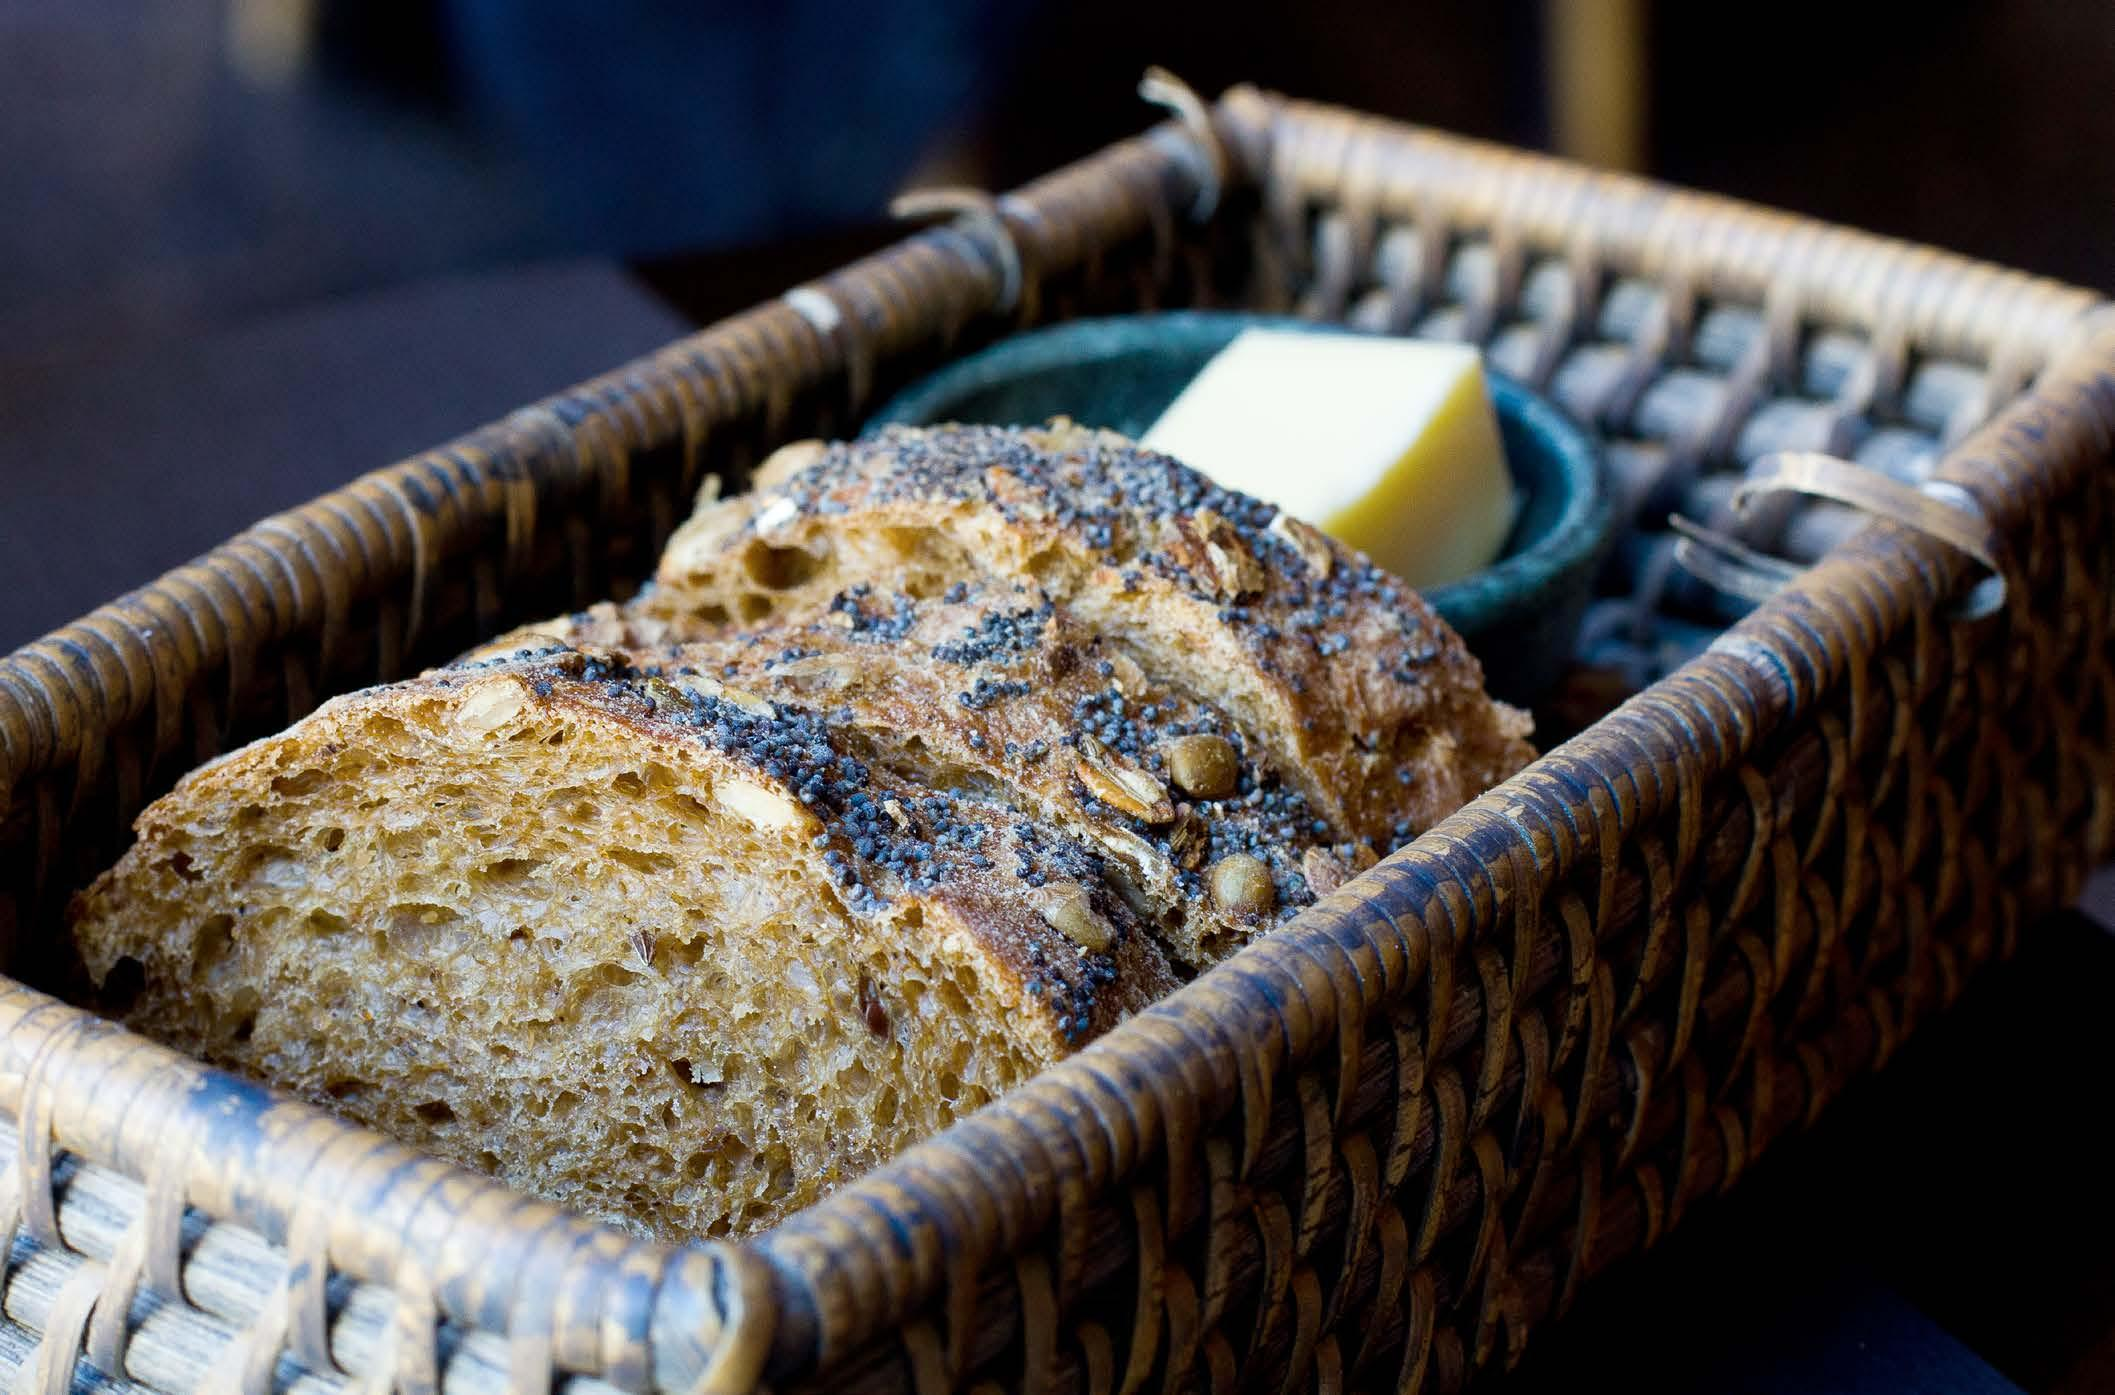
\includegraphics[scale=0.08]{depth_field_example1.jpg}
    }
    \subfigure[] {
                \label{fig:depth_field_example2}
                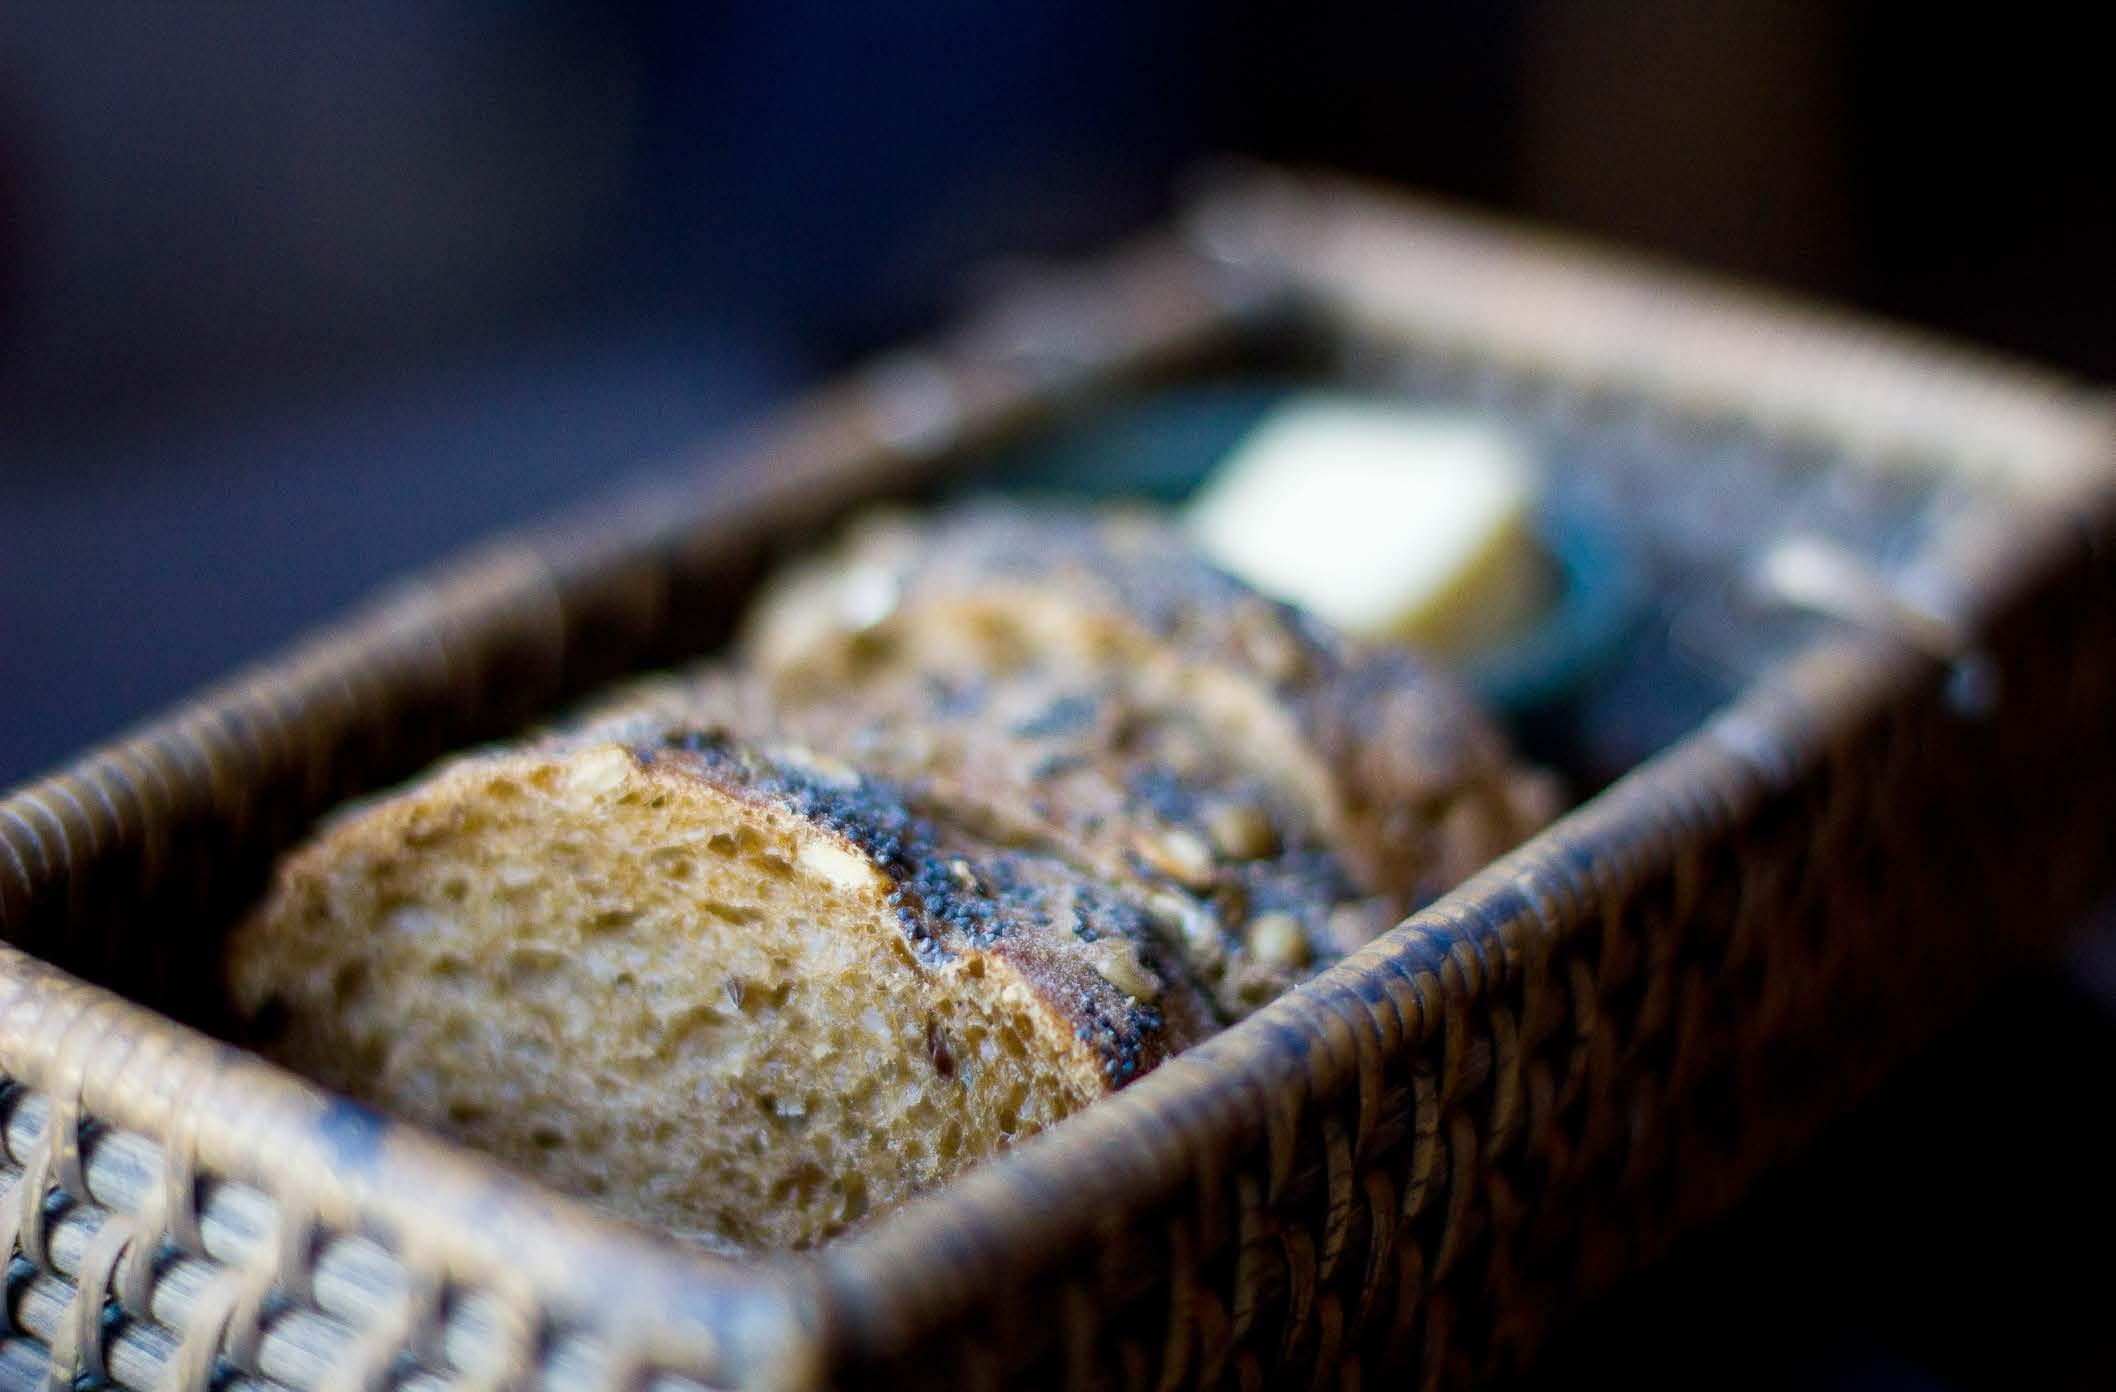
\includegraphics[scale=0.08]{depth_field_example2.jpg}
    }
  \caption{Difference between a shallow depth of field (a) and a wider depth of field (b). \cite{Kamps2012}}
  \label{fig:depth_field_example}
\end{figure}

\subsection{ISO}
\label{sub:iso}

This is the measure that defines the camera sensor sensitivity to the light \cite{Kamps2012}. Digital cameras tend to behave better in low light conditions with higher ISO values, which means that for higher ISO values, the camera's sensor becomes more sensible to light rays.
In digital cameras and mobile devices, the sensitivity can be adjusted if necessary. However, increasing the camera's sensitivity to the light might ruin a photograph due to the fact that it will introduce some digital noise in the image, as shown in Figure \ref{fig:iso_example}\footnote{\url{http://photographylife.com/what-is-iso-in-photography}}. To reduce this negative effect in the image, the use of high ISO values can be compensated with fast shutter speeds and low aperture values.

\begin{figure}[htbp]
        \centering
    \subfigure[] {
                \label{fig:iso1}
                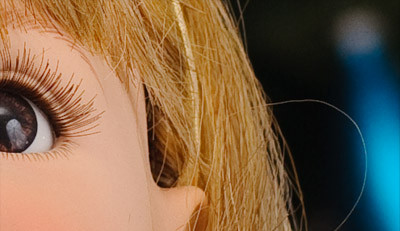
\includegraphics[scale=0.45]{iso_example1.jpg}
    }
    \subfigure[] {
                \label{fig:iso2}
                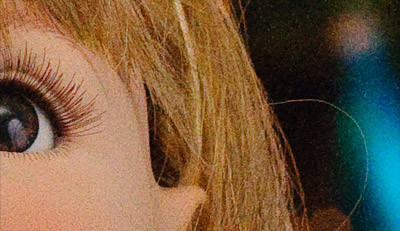
\includegraphics[scale=0.45]{iso_example2.jpg}
    }
  \caption{Difference between an image with ISO value of 200 (a) and 3200 (b).}
  \label{fig:iso_example}
\end{figure}

\subsection{White-balance}
\label{sub:white_balance}

It is a known fact that the human eye is more sensible to light variations than colour variations, therefore, when we see an object reflecting light, our brain instantly interprets the colour. This means that in areas of different brightness, our eyes adapt and interpret the same colour, although, to the camera they are not equal.
Since camera's are not capable of simulating the human brain, that is why white-balance is used in professional photography, in order to match the captured ambience light to what our brain would read \cite{Kamps2012}. Figure \ref{fig:white_balance_example} illustrates various examples of images with different tonalities that can be corrected adjusting the white-balance.

\begin{figure}[htbp]
        \centering
    \subfigure[Too cold] {
                \label{fig:white_balance1}
                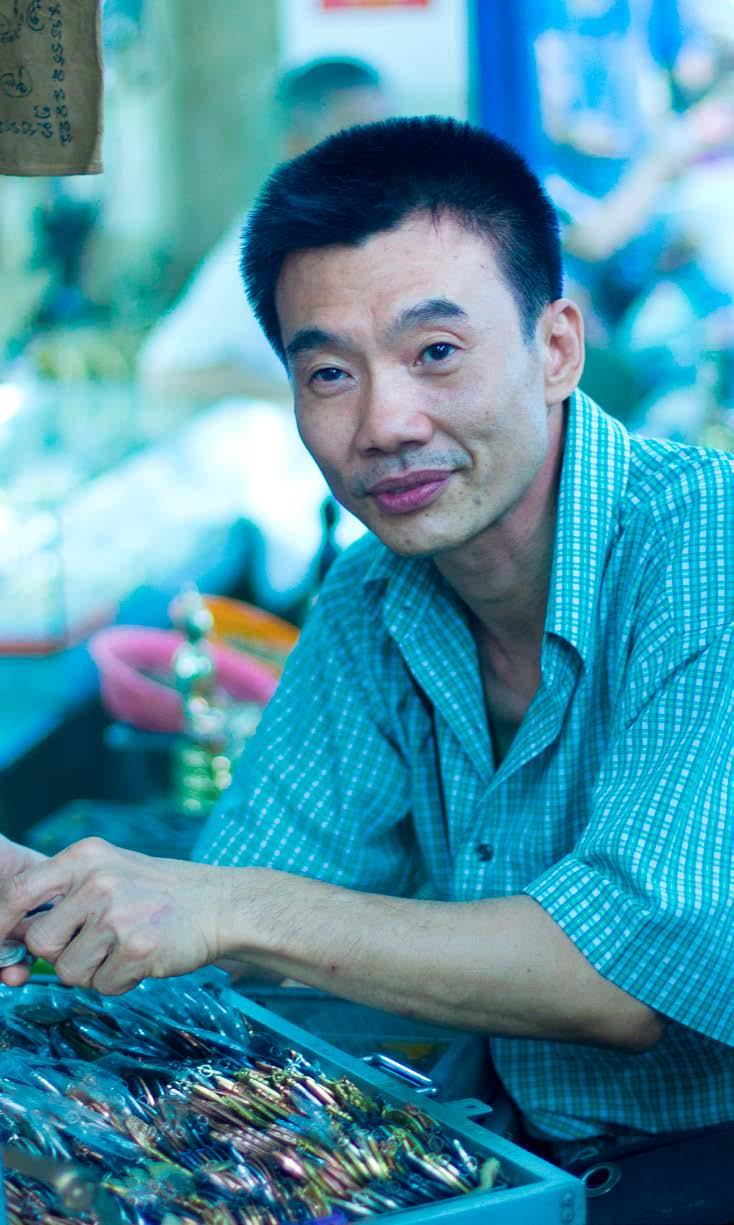
\includegraphics[scale=0.1]{white_balance1.jpg}
    }
    \subfigure[Well balanced] {
                \label{fig:white_balance2}
                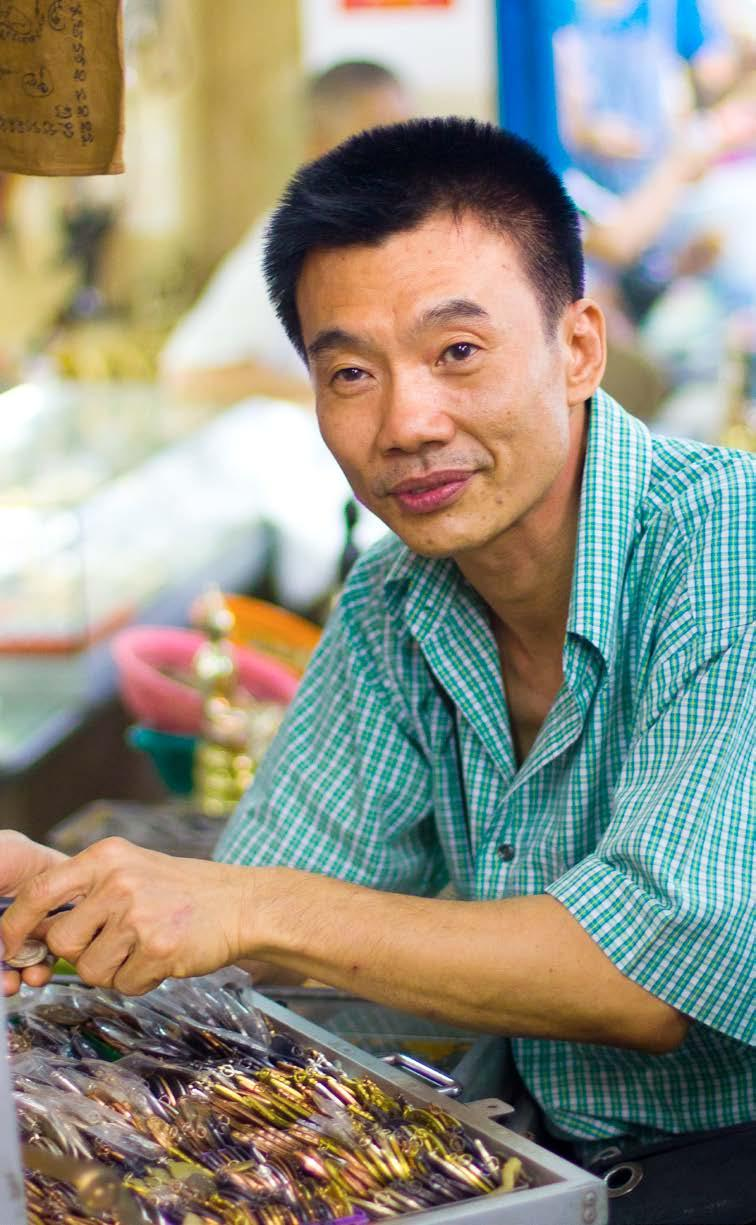
\includegraphics[scale=0.1]{white_balance2.jpg}
    }
    \subfigure[Too warm] {
                \label{fig:white_balance3}
                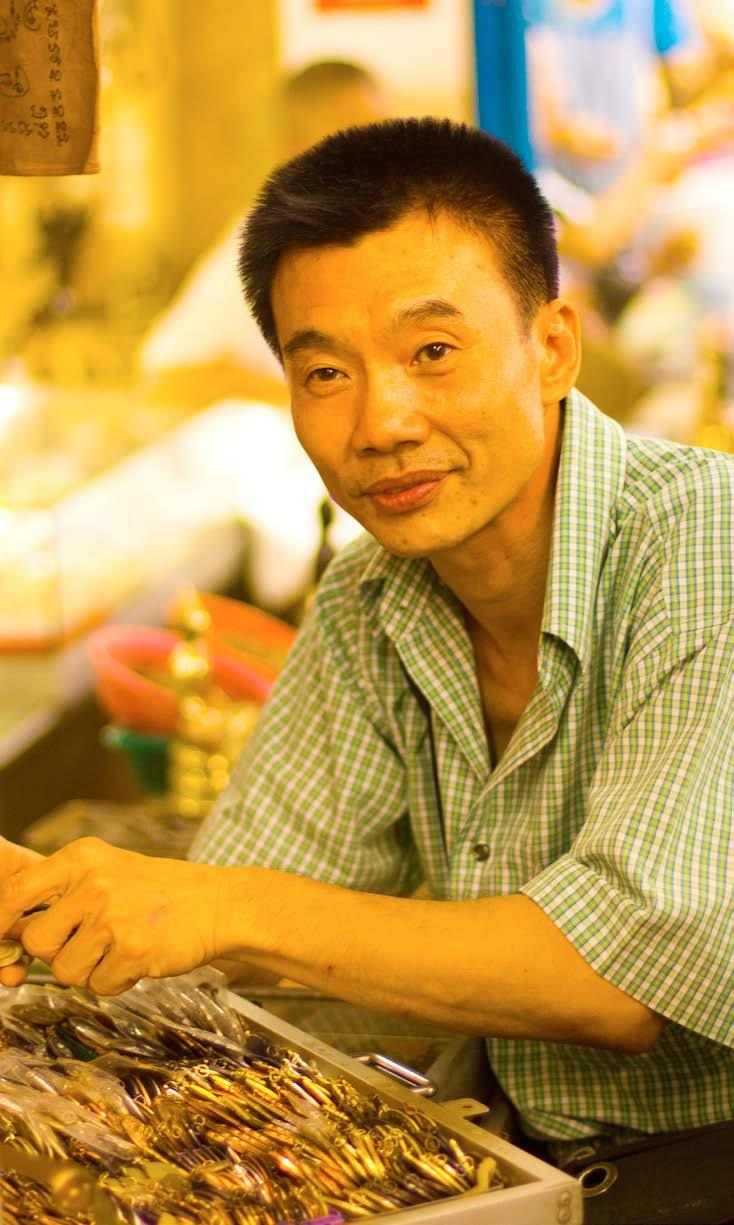
\includegraphics[scale=0.1]{white_balance3.jpg}
    }
  \caption{Three examples of white-balance applied to a photograph \cite{Kamps2012}.}
  \label{fig:white_balance_example}
\end{figure}


% ===============================================================
% =		    Processing techniques for photography				=
% ===============================================================
% # SECTION: Fundamental Concepts #



% # SUBSECTION: Processing techniques for photography #
\section{Processing techniques for photography}
\label{sub:photo_techniques}

\todo[inline]{rever paragrafo}
In early days, to render seascapes showing both the sky and the sea was impossible at the time using standard methods, due to luminosity range being too extreme. Photographers overcame these difficulties by exploring concepts such as the ones described in Section \ref{sec:concepts}. Exploring such concepts led to a development of new techniques, resulting in photographies with different properties. This chapter will describe some of these techniques and how they can be achieved.

%To take advantage of the most recent capturing technology, new techniques and add-ons are being created to obtain the most pure and stunning result without any kind of editing. These techniques are achieved by exploring lenses and other concepts, such as the ones described in Section \ref{sec:concepts}. This chapter will describe some of these techniques and how they can be achieved.


\subsection{Long-Exposure Photography}

Long-exposure (or time-exposure) photography exists since the popularization of photography. In the beginning, a person was obligated to stand completely immobile in front of a camera so that the final result would be as sharp as possible.
With this premise, long-exposure photography is a technique which involves taking a picture with a long shutter-speed \cite{Kamps2012}. This way the camera sensor will record more light while the shutter is open. With such long speeds the sensor cannot record moving objects, resulting in perfectly sharp capture of stationary objects and blurring or obscuring of moving elements.
This technique is more successful under low light conditions due to the time that the sensor is exposed to light, but this can be suppressed by using special filters for the lenses. By taking so long to close the shutter, the sensor keeps absorbing light creating a brighter photograph producing a near daytime effect.
This technique made easier for professionals to photograph at night, and gave form to new types of photography such as light painting where a person with a light source can draw paths in the air. Being more sensitive to light, while the shutter is open, the sensor records all the paths drawn resulting in an image where the paths form a continuous line and the person or object moving the light source is obscured, as shown in Figure \ref{fig:long_exposure_example}\footnote{Source: (a) \url{http://www.hongkiat.com/blog/light-painting-artworks/}, (b) \url{http://www.flickr.com/photos/awfulsara/35403447}}. Such technique can also be achieved by manually blurring specific areas of a photo, using image editing software.

\begin{figure}[htbp]
        \centering
    \subfigure[] {
                \label{fig:long_exposure_example1}
                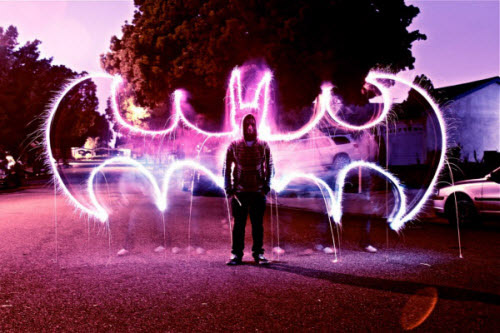
\includegraphics[scale=0.4]{long_exposure_example1.jpg}
    }
    \subfigure[] {
                \label{fig:long_exposure_example2}
                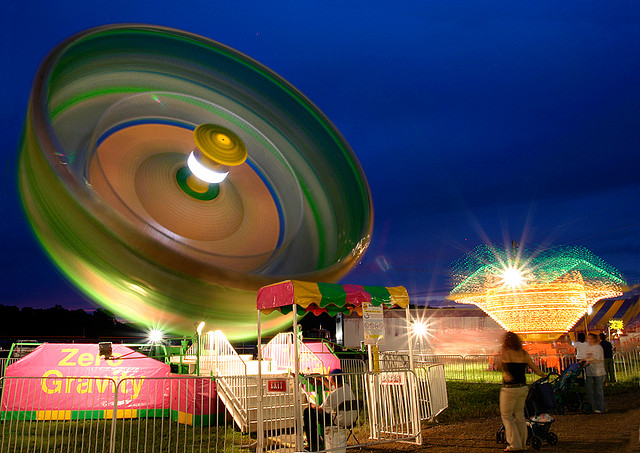
\includegraphics[scale=0.294]{long_exposure_example2.jpg}
    }
  \caption{Examples of Long-Exposure Photography. \cite{Kamps2012}}
  \label{fig:long_exposure_example}
\end{figure}

\subsection{High Dynamic Range Imaging}

\todo[inline]{rever secçao}
Although there is a big improvement in the technologies related to photography, cameras still have a problem of not being able to perceive colours the same way as the human eye. Due to the inability of digital cameras to correctly perceive a scenes luminosity, it is possible to incorrectly record colours and lose information in lighter or darker areas accordingly to the exposure. High Dynamic Range Imaging is based on a capture that can represent a more accurately range of intensity levels found in scenes compensating this problem.
In photography, this technique is achieved by taking multiple Standard Dynamic Range (SDR) photographs of the same scenario with different exposure values that can vary depending on the device. After taking all the samples, the process consists in combining all the raw data of over-exposed and under-exposed areas in one image. By doing this, the image will result in a photograph with a broader tonal range, as shown in Figure \ref{fig:hdr_example}\footnote{Source: \url{http://www.flickr.com/photos/wetworkphotography/7437783578}}.

Although cameras already have enough computational power to perform this techniques, \citeauthor{DebevecPaulE.;Malik} \cite{DebevecPaulE.;Malik} also proposed a method of recovering high dynamic range radiance in photographs taken with conventional image equipment. 
As expected, multiple photographs are taken with different amount of exposure. Using these photographs as samples, they recover the response function of the imaging process using the assumption of \emph{reciprocity}, which can be defined by a sensor response to the total exposure (i.e. $itensity x time$ controlled by the aperture and shutter-speed (Section \ref{sec:concepts})).
Having obtained a response function, the luminosity value of each pixel is computed using all the available exposures, in which its value is closer to the middle of the response function.

Another approach taken by \cite{Vavilin2011} involves three cameras, side by side, in the same optical axis that can be seen in Figure \ref{fig:hdr_camera}. Each of this cameras takes a photograph with different exposure values, taking a first picture underexposed, a second picture with the normal exposure, and a third picture overexposed. These three images are overlapped and merged, reconstructing information lost in overexposed and underexposed areas.

\begin{figure}[htbp]
        \centering
    \subfigure[Non HDR] {
                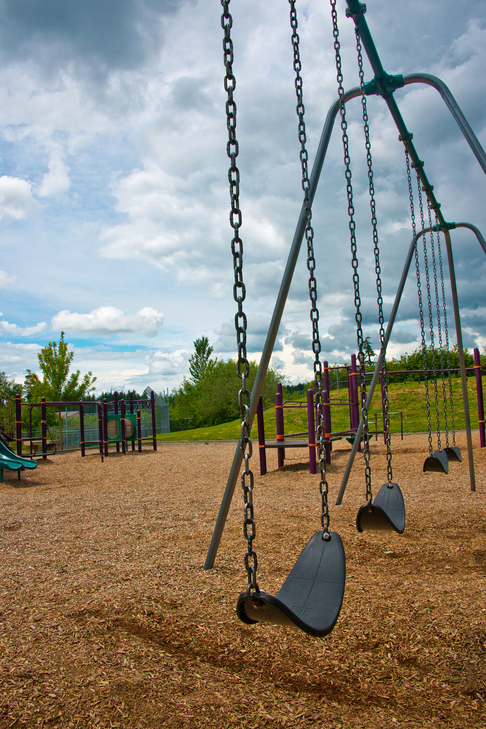
\includegraphics[scale=0.18]{hdr_example1.jpg}
    }
    \subfigure[HDR] {
                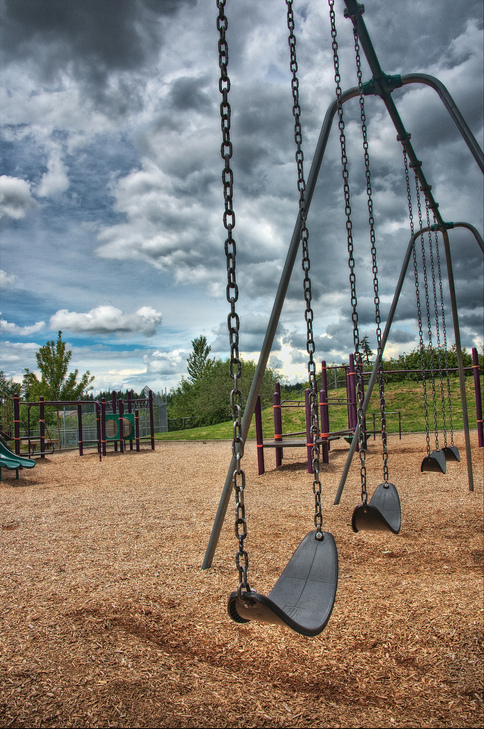
\includegraphics[scale=0.18]{hdr_example2.jpg}
    }
  \caption{Example of a picture taken with High Dynamic Range (b) versus the same picture with Standard Dynamic Range (a).}
  \label{fig:hdr_example}
\end{figure}

\begin{figure}[htbp]
	\centering
	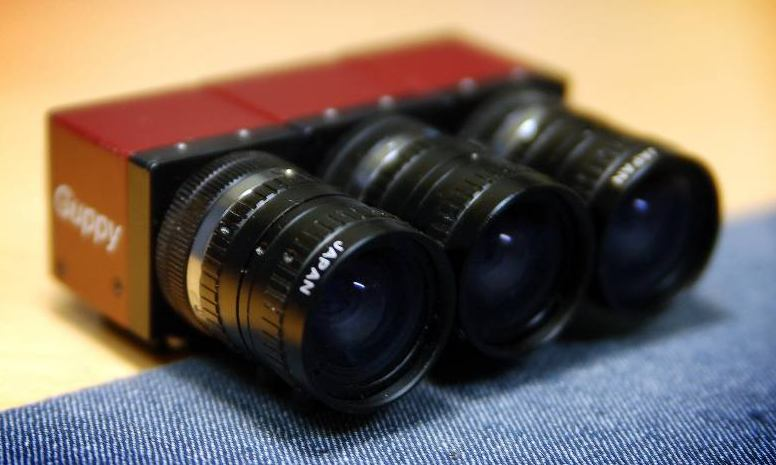
\includegraphics[scale=0.15]{hdr_camera.png}
	\caption{Image of the three cameras aligned side by side \cite{Vavilin2011}.}
	\label{fig:hdr_camera}
\end{figure}

\subsection{Panoramic Photography}

\todo[inline]{rever secçao}
Panoramic photography is a technique that creates an image with an enlarged field of view which approximates or exceeds the human eye (160º by 75º). Among specialized methods and devices, one of interest is the use of Catadioptric cameras and lenses. These cameras are based on a system of lenses and curved mirrors that allow a field of view of 360º over a single viewpoint, bypassing the need of horizontal panning as it occurs with other methods. Since it uses mirrors and lenses, the light rays bent preventing any kind of distortion or chromatic aberration. Without the need of computation, another advantage is the use of this cameras for video shooting of 360º panoramas. 
There are on the market some add-on lenses for mobiles devices that make this technique possible, such as GoPano micro (Figure \ref{fig:gopano}).

There are also methods to generate panoramas by stitching multiple horizontal images through software.
\citeauthor{Brown2006} \cite{Brown2006} described an algorithm that would generate a graph to recognize individual panoramas by find all pairwise image overlaps using feature-based methods. After finding all images with matching features, it would readjust the rotation of the images to generate a panoramic image. This method would be insensitive to the ordering, orientation, scale and illumination of the input images. After

\citeauthor{Szeliski} \cite{Szeliski} describes methods to create full view panoramic mosaics. He first describes a method of generation cylindrical panoramas with a sequence of images taken by a camera mounted on a levelled tripod. This algorithm consists in estimating consecutive horizontal and vertical translations for each image. To recover the translational motion, the incremental translation is estimated by maximizing the corresponding points between them. It would be possible to convert an image to 2D spherical or cylindrical coordinates for a known tilting angle but it would not minimize the error between two images, therefore, this method can only handle the simple case of pure panning motion.

Secondly, \citeauthor{Szeliski} \cite{Szeliski} introduced an algorithm that does not need a set of pure horizontal images. Instead, as long as there is no strong motion between sampled images, there are no constraints on how images are taken. This makes photographs taken by hand-held devices without a tripod a reliable source for creating panoramas. According to \citeauthor{Szeliski}, the center point of the sampled images can be described in 3D by a set of matrices which correspond to the image plane translation, the focal length scaling and a 3D rotation matrix. After estimating the mean focal length of the images and rotation matrix, they can stitch the images in a 3D dimensional space.
Since it is made by stitching multiple images, the final product presents distortions at the north pole. This is because of a necessary warp to cylindrical or spherical coordinates (Figure \ref{fig:panoramic_example}) to have a full view of the panorama without using a specialized viewer.

\begin{figure}[htbp]
        \centering
    \subfigure[] {
                \label{fig:gopano}
                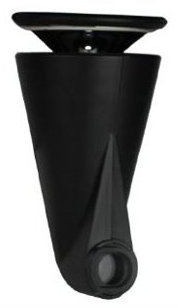
\includegraphics[scale=0.3]{gopano.jpg}
    }
    \subfigure[] {
                \label{fig:panoramic_example}
                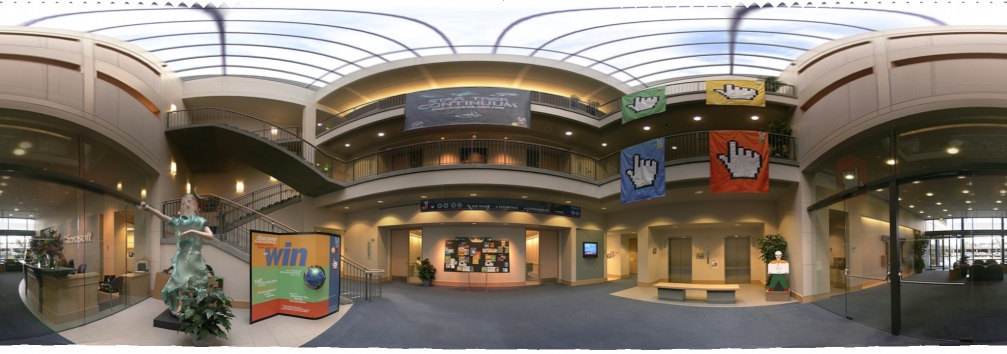
\includegraphics[scale=0.45]{panorama_example.jpg}
    }
  \caption{Image of attachable lens for iPhone, GoPano micro (a), and panorama made by the algorithm described at \citeauthor{Szeliski} \cite{Szeliski} with distortion at the north pole.}
  \label{fig:panoramic_image}
\end{figure}


% # SUBSECTION: Image capturing and processing apps #
\section{Image Capture and Processing}
\label{sub:capturing_processing}

Since the first attempts to capture a scenery, to its popularization in the XIX century, the world of photography has suffered improvements, that still shock many professionals in the business. Since the upgrade of analogue cameras to the digital world, the use of negatives and dark rooms to new techniques like tilt-shift and HDR imaging, the current market has been increasingly overwhelmed by mobile devices and their ability to easily dethrone today's digital cameras. Proof of this fact is the wide range of applications related to photography available in mobile devices application stores like Google Play and App Store. A more professional objective than others, throughout this chapter, it will be discussed some of those applications for image capturing and processing. Along with these applications, research that has been done in this field will also be discussed.

\subsection{Image Capture}

The advancements in mobile devices created a new type of market. Due to this virtual market available for any Android or iOS user, the number of mobile applications are constantly increasing. Camera related applications are no exception to this rule. In both markets there are many applications fully capable of capture images that were designed for social networks or include special features. We will start by presenting the default applications in both Android and iOS systems, and other applications found on both of those markets, ending with a discussion comparing all of them.

\subsubsection{Android and iOS Native Applications}

By default, the newest mobile operating systems, already have an incorporated application to take photos. For example, on iOS, the default application is rather simple. It has very few customization options for a user that has more knowledge in the area, although, it is possible to record videos and choose between full screen photos or photos with a squared format, using one of the two cameras available, with or without flash. Besides these, the iOS native application offers a short-cut to access the device's gallery.

On the other hand, android's native application is a flexible alternative. It offers access to more advances functionalities in the likeness of today's digital cameras.
Some of these options include messing around with ISO and exposure values, white-balancing, contrasts, and choose the resolution of the final product. Also enables the user to choose the correct capture mode for the moment, e.g. sports mode, indoor, portrait, etc.
Android's application adds meta-data tags to the image which may include GPS location and renames the file according to that location. It becomes more user friendly, when displays a grid on the screen. This grid serves as a guiledine so the user can position the object in the frame. Despite all the options, one of the most useful features is the anti-shake system that applies corrections onto an image to compensate the user's movements.


%\subsubsection{Instagram (iOS)}

%With already a notorious percentage of popularity and very centred in social networking, Instagram is an application that offers the main features of a native application. Some of these features include the possibility of taking a photograph or record a video and choose between between the front and rear camera, if they both exist on the device. With direct access to the device’s gallery in both modes, the shooting mode, in similarity with Android’s default, shows a grid in the display, and control options for flash.
%The presence of menu bars at the top and bottom of the screen reduces the space available to preview the shoot and maintains a squared shape for both the preview and the shoot taken, as shown in Figure X.


\subsubsection{Photoshop Express (iOS)}

Tool developed by Adobe \cite{Photoshop} that has a shooting mode with some extra features in comparison with the native application.
Having a preview of the image taken is an interesting feature to be used in a more professional context, allowing the user to decide if it is an usable photo before saving it in the gallery.
Although in most of the available applications the zoom feature is already a given, in Photoshop Express it can be controlled by an horizontal slider. The fact that it is always visible, the user understands how to make zoom more easily comparatively to default applications, where the zoom can be done by performing a pinching action on the screen. The pinching action might not be very intuitive for someone using the application for the first time, therefore, an horizontal slider as the one presented in Photoshop Express might be a good alternative.

\subsubsection{Photosynth (iOS)}

Photosynth, developed by Microsoft \cite{Photosynth}, was created to support a social network centred in creating and sharing panoramic photos. The social features will not be described since they are not the main topic of this thesis.
Regarding the image capturing abilities, this application allows the user to create a software generated panoramic image. The device displays a 3-dimensional spherical space that rotates with the user's movement. As soon as the capture starts, Photosynth automatically captures the initial scene and all the adjacent scenes while the user is rotating. After the capture, this application identifies specific features in one photograph and matches with other photographs features and by analysing the position of matching features identifying photographs belong on which side of others. 
To visualize the panoramic image, the stitched images are displayed in a 3-dimensional spherical space similar to the one presented on the capture display, with the particularity that the user must scroll to see the final result. Outside the application, previewing the image in the gallery, it presents some deformations due to spherical transformations applied to the sampled photos. 


\subsubsection{Camera FV-5 (Android)}

Camera FV-5 \cite{FV5} is one of the most complete applications for photography in the Play Store. Although it has a screen with many options and information, it is what most resembles to a digital camera display. It offers full control over exposure, ISO and white-balance. Exposure can be manually selected by the user or, alternatively, she can choose between modes that automatically determine exposure values based specific regions of the image displayed in viewfinder. 
Multiple focusing modes are available, that allow macros, setting the focus to infinity or taping the display and select the object to focus.
More related to camera utilities, multiple flash modes are available including a flashing mode that fixes red eyes on photos, and other shooting utilities that include a shooting timer, image stabilization and burst mode.
For a more inexperienced user, default programs with pre-defined exposure settings can be used.
The most interesting trait are the indicators in the viewfinder that display values of exposure time, aperture, ISO, battery remaining and how many photos are in buffer (Figure \ref{fig:FV52}).
Camera FV-5 allows control over the available parameters, recreating some photographic techniques. Due to hardware issues, these recreations are the result of software emulation and not from lens adjustments thus reflecting in the quality of image taken.

\begin{figure}[htbp]
        \centering
    \subfigure[] {
                \label{fig:FV51}
                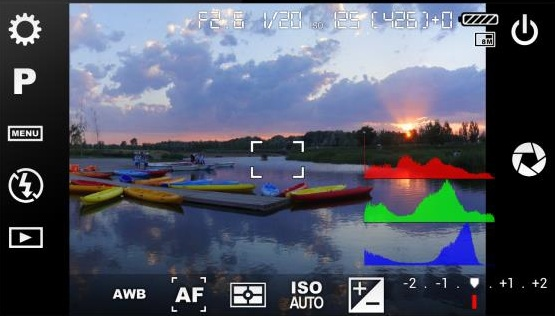
\includegraphics[scale=0.4]{FV51.jpg}
    }
    \subfigure[] {
                \label{fig:FV52}
                
\includegraphics[scale=0.45]{FV52.jpg}
    }
  \caption{Interface of Camera FV5 (a) and interface indicator (b) of aperture, exposure time, ISO, etc \cite{FV5}.}
  \label{fig:FV5_image}
\end{figure}


\subsubsection{SketchCam}

SketchCam \cite{Labrune} appears as a research project that uses a different approach towards mobile devices in photography. With a touch screen, it enables children to capture images by sketching the area of interest on the display. 
Using this approach, it allows the user to become more selective towards the scenario in front of her. It enables creativity in a way that the user may be able to create different frames for the picture that is being taken.  After selecting the point of interest in the view display, it creates an object that can be used for future collages. This may help teaching the basic concepts of composition and photo editing by using a different display. 


\subsubsection{Frankencamera}

Although there are many mobile devices with capabilities to take photos, most of them don't take full advantage of the imaging hardware and offer a highly simplified API. The programmer can't control the camera exposure time or retrieval of raw sensor data. Motivated by these problems, Frankencamera \cite{Szeliski2012} is an open-source architecture with a custom-built camera based on Linux and gives full control of the hardware to the programmer through C++ language. These architecture consists in an application processor, a set of photographic devices such as flashes and lenses, and one or more image sensors, each with a specialized image processor, forming a tightly coupled pipeline to coordinate all elements. All sensors, devices and parameters that describe the capture and post-processing of a single output image, can be programmed through its API allowing a mechanism to precisely manipulate the hardware state over time.

Being a custom made platform, it brings some advantages towards closed platforms. One of these advantages is the ability to take long-exposure photos without a tripod. Using an embedded gyroscope, the camera will stream full-resolution raw frames that will be stored, only if their gyroscope tags indicate a low motion when the frame was taken. 
Another useful application is the creation of panoramic photos with extended dynamic range. In most devices, the user has to take various individual photographs and stitch them together on a computer, but with this system it is possible to individually set the exposure time of each shot creating a panorama with extended dynamic range and previewing the result instantly.

\subsubsection{Discussion}

All commercial applications and research projects share the most basic features that should come embedded in any system capable of taking photos. These features include access to a gallery, control over flash, control between frontal or rear camera, an auxiliary grid and control over zoom.
%In order to dethrone digital cameras, stock applications such as the ones that come by default with Android and iOS, started that process of mass dissemination of a portable, simple and completely capable option to take casual photos. 
Android applications, comparatively to iOS, offer more control over the device's hardware, such as shooting mode, resolution and image quality, aperture and ISO values. Allowing almost full control of the hardware to the user, is a very important feature that must taken in consideration when developing an application to take photos. Given this fact, Android became a more reliable platform for users that want to use their mobile device for something more than casual photos.

With some interesting features, Camera FV5  is one of those applications for amateur photographers that presents a similar interface to a digital camera with a possibility of adjusting some photographic parameters and introduces the emulation of photography techniques.
Interesting features that should be noted on Photosynth is the way the application handles the creation and preview of panoramas, where it detects and stitches in real-time, a sequence of consecutive photos by matching features on a 3-dimensional spherical space.

As research projects, SketchCam and FrankenCamera can go beyond what is available on regular systems. Although designed for kids, Sketchcam presents a system with a very different way to interact with the user in how she takes a photo. Selecting the point of interest by sketching a continuous path and giving form to different shapes of frames in a display with a live video feed, can be handy when a user only wants to emphasize a region or object in the viewfinder.
Frankencamera allows computational photography to take a step further. It is the perfect example of what is possible by taking full advantage of a device capabilities. It allows to take long-exposure photos using the available gyroscope proving that better photos can be taken using multiple sensors available.


\subsection{Image Processing}
\todo[inline]{rever secção}
Image processing encompasses the task of altering images, whether they are digital photographs, traditional photochemical photographs, or illustrations. During recent years, image retouching of photographs have gained an important role in the industry and more recently, image editing has became available to anyone. Chosen by some as primary cameras, mobile devices with embedded cameras also have a role to play on this subject. Research has shown that users often do little editing of photos after the shot has been taken \cite{Brewster}, and for that reason mobile devices now offer applications for both capturing and editing images. This section will describe some applications that apply some image editing principles and tools.
 
\subsubsection{Android and iOS Native Applications}

Being multifunction system, iOS already bring functionalities for image editing. Being a unique system for all devices that support it, automatically all devices have some basic tools that can be used in photographs.
These basic tools include image rotating and image crop where a user can define which part to crop and select the proportion of the rectangle where the crop will be applied.
Since iOS doesn't have an option to remove the red-eye effect, a user can later remove it by editing the photo and selecting the eye affected. More related to image effects, iOS offers a set of filters that can be applied to a photo.
to facilitate the user, iOS has an option of auto enhance, where it readjusts the images white-balance and automatically detects and removes the red-eye effect (Figure \ref{fig:ios_edit_image}\footnote{Source: \url{http://www.shortcourses.com/images/b4ch6/eerie.jpg}}).

Android on the other hand, comparing with previous versions, has a full set of tools available for image processing. Besides the sharing the same options as iOS, it has a a group of advanced adjustments that can be applied to a photo \cite{Sharon}. With these, a user can readjust exposure levels, contrast, hue, etc. In cases where only a specific part of a photo needs to be adjusted, Android allows local fine-tuning where a user apply corrections to multiple selected areas. At any point within the editor, a user can drag down from the top to view the original photo and save the edited image specifying the desired size and quality.

\begin{figure}[htbp]
        \centering
    \subfigure[] {
                \label{fig:ios_edit1}
                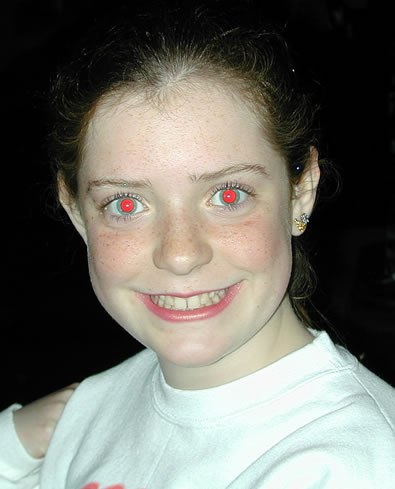
\includegraphics[scale=0.35]{ios_edit1.jpg}
    }
    \subfigure[] {
                \label{fig:ios_edit2}
                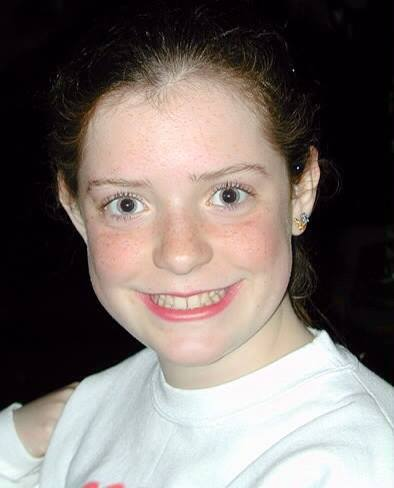
\includegraphics[scale=0.35]{ios_edit2.jpg}
    }
  \caption{Image (a) before and (b) after applying the auto enhancing tool. It is possible to see that the red-eye remover only darkens the red area and does not take in account the real colour of the eye.}
  \label{fig:ios_edit_image}
\end{figure}

\subsubsection{PixelNote}

PixelNote \cite{Laput2013} is an iPad application for photo edition that works through a multimodal interface combining voice recognition and direct user interaction to manipulate images. It uses natural language is used to express how to modify an image and sketching to localize these changes to specific regions. Using the two inputs, a user can select and tag an object with a voice command that can be used for future identification through voice recognition.

The speech recognition technology converts the voice into character strings that PixelNote can process. First the strings are by a local speech recognition engine that is trained for a specific set of words selected from a user study. When the system encounters words out of the expected vocabulary, the recorded voice data is sent to a remote speech recognition server. When all else fails, PixelNote shows a gallery with options that may be appropriate . Thus, this fallback system allows the user to also learn the vocabulary of the system while editing the image successfully.

\subsubsection{Discussion}

iOS and Android default applications represent two extremes of what is possible in terms of image editing on a mobile device. Other applications such as Photoshop Express (Android and iOS), Photo Editor (Android) or Camera Awesome (iOS) have the same functionalities as Android's default application. Being relatively advanced in photo editing, Android introduces the notion of local fine-tuning to an image where a user can apply different corrections to localized areas of an image.
As a research project, PixelNote explores different ways of interacting with mobile devices. Using voice recognition with sketching on localized areas, PixelNote enables object selection and tagging, and correction of specific areas in an image by recognizing specific voice commands. This project shows that is possible to extend an application capabilities for photo editing, exploring different types of interaction reducing the difficulties of such a task on a small and portable screen.

Both multimodal interfaces and localized corrections, are features that should be taken in consideration when thinking of how to apply effects and interact with small screens has the ones in mobile devices.

%------------------------------------------------------------------------------------------------------------------
%------------------------------------------------------------------------------------------------------------------
%------------------------------------------------------------------------------------------------------------------

% # SECTION: Avaliação de Fotografia #
\section{Image Evaluation}
\label{sec:photo_eval}
To understand aesthetic problems, \citeauthor{Hoenig2005} \cite{Hoenig2005}, described and formalized a set of theorems and components that could provide a measurable basis for aesthetics.
According to the author, in 1933, George David Birkhoff came up with a formula that encapsulated his insights into a aesthetic value, described by $ M = Order/Complexity $. This represents the reward one gets, by experiencing orderliness while putting effort in focusing details, giving higher aesthetic value to beauty over complexity. Birkhoff's concept sparked interest of computer scientists in aesthetics, creating the term computational aesthetics. This term is described as a set of computational methods that can make applicable aesthetic decisions in a similar fashion as humans can.

%A professional photographer might have a good equipment, the perfect light and a good control over exposure, but one key feature is the composition of the picture. Many of the rules of composition used by photographer have been copied from classical painters.
%Photographers have the challenger of taking an interesting photography, and a good composition encourages the viewers eyes to roam around the image and capture hers attention.
%There is no recipe for a good composition, and for that reason a photographer must have in consideration of how an image is read by the majority of population. The inherent tendency to sweep an image from left to right, and from top to bottom, with the knowledge of how the human eye reacts to colour, luminosity, directing lines are facts that are taken in account when shooting and when evaluating an image. This section contains two subsections where this concepts will be explained in the first one and some approximations of their use for evaluation will be introduced on the later.

% # SUBSECTION: Regras de Composição #
\subsection{Composition Rules}
\label{sub:photo_rules}

\todo[inline]{rever parágrafo}
To obtain aesthetic results, photographers follow certain rules of composition that are the result of centuries of artistic development. These rules are now considered as rules of thumb and serve as guidelines. Following these guidelines helps obtaining pleasant results but this is not absolute. Professional photographers also criticize them and defend that one must know when to break them.
Being such a subjective topic, there is no recipe for a good composition and professional photographers always have the final call when taking a photo. This section describes some of the rules that captures the viewers attention and can be used in computational aesthetics.

\subsubsection{Colour Balance}
\label{subsub:colour_balance}

Although a good photography is dependent on the subject that is being captured, colour has a major impact in creating a certain mood and empathy with the viewer. 
%In digital photography what is captured is the transmitted light and not the reflected light, the primary transmitted colours are composed by red, green and blue (RGB), and consequent secondary colours obtained by merging this three components. 

It is rare for a colour to be isolated in a photo shoot, and depending on the colour palette, a different relation between them will be established. These relations can create similar or different emotions that can be explored in a composition \cite{Santos}.
A relation created by two complementary colours gives a sensation of balance, but if both colours have different luminosity values, the less luminous colour must be present in a greater amount comparing to its complement (Figure \ref{fig:colour_balance_image}).
To evoke a mood and arouse emotions, each colour has its own meaning that can be interpreted in different ways by different cultures. For the western civilization, yellow symbolizes cheerfulness, joy and optimism, but for the eastern civilization, it is related to the imperial kingdom and symbolizes something sacred. On the other hand, in the Egypt, it is a colour for mourning.

\begin{figure}[htbp]
    \centering
	\label{fig:colour_balance_example}
    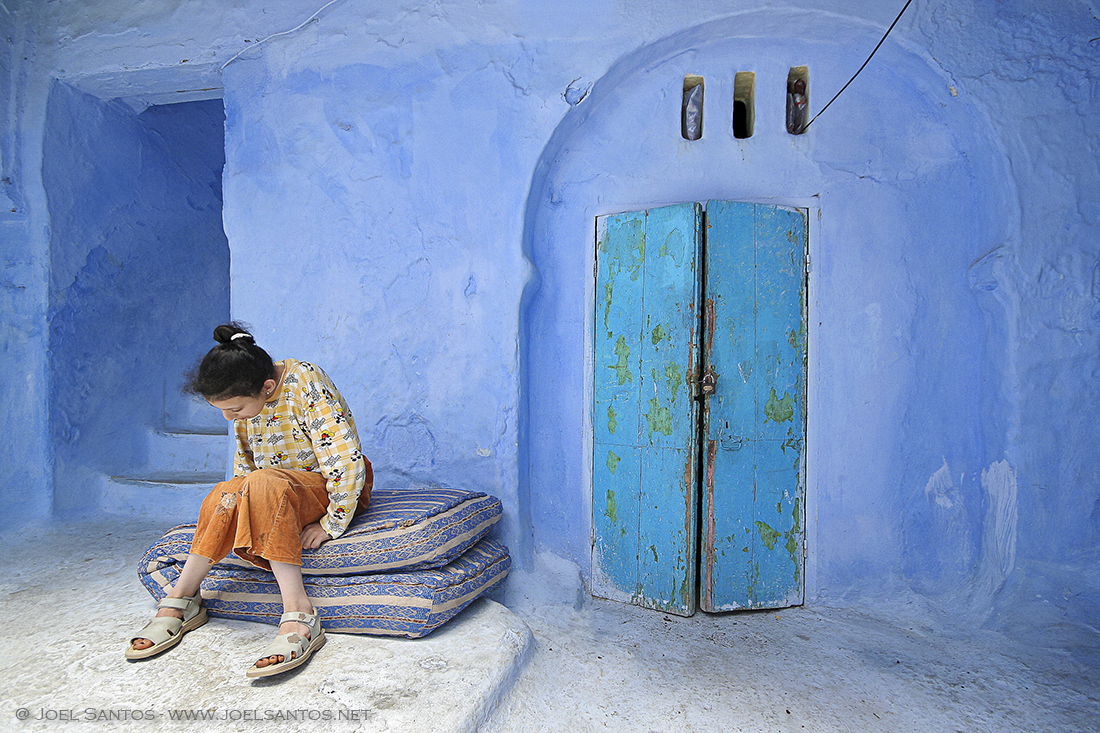
\includegraphics[scale=0.3]{color_balance_example.jpg}
  \caption{Image of two complementary colours balanced in a frame. \cite{Santos}}
  \label{fig:colour_balance_image}
\end{figure}

\subsubsection{Rule of the Golden Section and Golden Spiral}
\label{subsub:golden_section}

There are rules used by many photographers, artists, architects, and considered to obtain very appealing results. The golden section rule is based on the golden average. This value can be achieved from a division between two consecutive numbers in a Fibonacci sequence. For example, defining the sequence [8,13,21] as a subsequence of the original Fibonacci, dividing 13 by 8, and 21 by 13 will result in a ratio, that in the limit, will be equal to the golden number (i.e. $\approx 1.6180339$). This golden number is what defines a golden section \cite{Santos}. 

This section, which is believed to be aesthetically pleasing, consists of a group of rectangles in which the ratio of the longer side to the shorter is equal to the golden ratio. It is possible to draw a logarithmic spiral whose growth factor is equal to this ratio, called the golden spiral, which converges to the smallest rectangle in the section. 

Using this golden ratio, one can form a grid dividing the golden section in 1.6 to 1 parts. Applying this division to a golden section, we obtain a grid as in to Figure \ref{fig:golden_section2}, where the intersection of the lines indicate imaginary points where the main subject should be located. From this point onward, these imaginary points will be treated as \emph{power point}. 

%With this concepts, it is possible to create a guideline based on the golden spiral where the \emph{power point} or a grid 
%With this concept, it is possible to create a grid formed by the intersection of vertical and horizontal lines that pass through four specific points. The points correspond to \emph{power points} obtained by converging a golden spiral from each vertex of the golden section (Figure X). This grid will result in a guideline with reference lines and imaginary points that indicate where the main subject of the scene should be located, usable in portrait and landscape mode.


\begin{figure}[htbp]
        \centering
    \subfigure[] {
                \label{fig:golden_section2}
                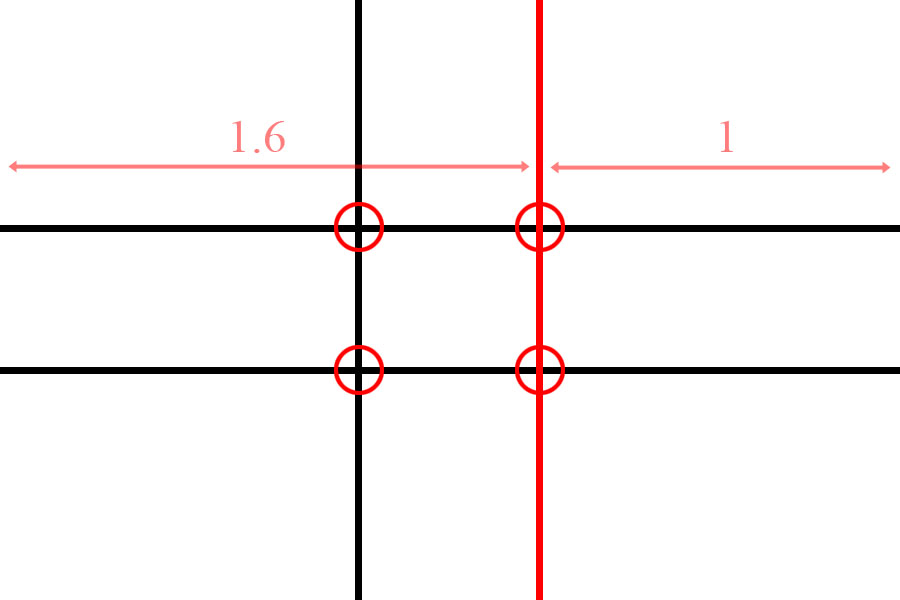
\includegraphics[scale=0.2]{golden_section2.jpg}
    }
    \subfigure[] {
                \label{fig:golden_section1}
                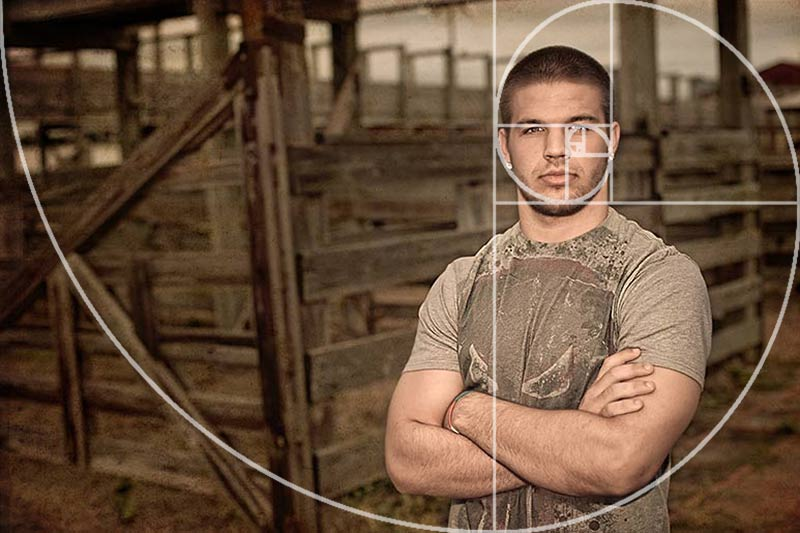
\includegraphics[scale=0.2]{golden_section1.jpg}
    }
  \caption{Guidelines formed from dividing the (a) golden section in 1.6 to 1 parts and from (b) the golden spiral.}
  \label{fig:golden_section_image}
\end{figure}

\subsubsection{Rule of Thirds}
\label{subsub:rule_thirds}

The rule of thirds is based on the golden section \cite{Santos}. While this last one results in a guideline where the \emph{power points} respect the conversion point of a golden spiral, the rule of thirds consists in dividing the rectangle in nine equal parts. The scene is divided in thirds both horizontally and vertically with power points at the intersections.
Being a derivation of the golden section, the fundamental concept of where the object should be, remains the same. The main subject should be positioned in one of the \emph{power points} and along the the lines, as shown in Figure \ref{fig:rule_of_thirds_image}.

\begin{figure}[htbp]
    \centering
	\label{fig:rule_of_thirds_example}
    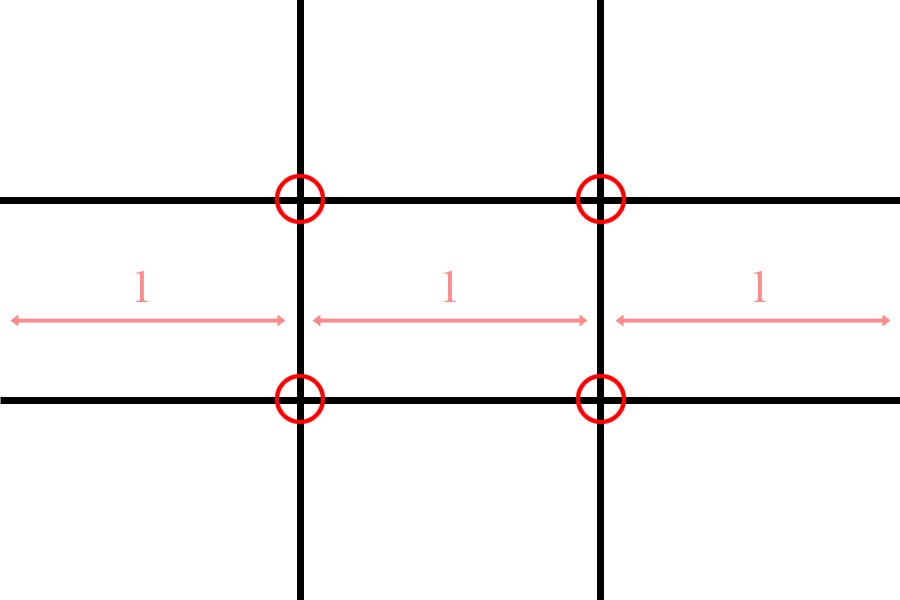
\includegraphics[scale=0.2]{rule_of_thirds.jpg}
	\caption{Guidelines of the rule of thirds with nine equal rectangles and respective \emph{power points} circled in red.}
	\label{fig:rule_of_thirds_image}
\end{figure}

\subsubsection{Triangles and Golden Triangles Rule}
\label{subsub:rule_triangles}
The most common shape of composition in a portrait is that of a triangle, imagining a portrait with the head being the peak and the width of the body being the base.

The golden triangles rule uses a group of triangles that follow the proportions described by the golden section. Using a golden section, we draw a diagonal line between two corners of the rectangle and connect a perpendicular line to each of the remaining corners. In some cases, this can be simplified to only one perpendicular, having only one power point in the intersection with the diagonal line and a suggestive region in the frame to place the elements \cite{Santos}.

\begin{figure}[htbp]
    \centering
	\label{fig:golden_triangle_example}
    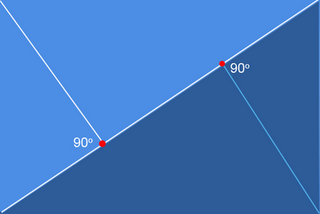
\includegraphics[scale=0.5]{golden_triangle.png}
	\caption{Guidelines obtained by the golden triangles rule.}
	\label{fig:golden_triangle_image}
\end{figure}

\subsubsection{Usage of leading lines}
\label{subsub:leading_lines}
\todo[inline]{rever, acho que so mudei o primeiro paragrafo e adicionei a ultima frase}
Lines can be used implicitly by creating an imaginary line between two subjects in a picture, or explicitly, like the edges of a building. In the perspective of \citeauthor{Kamps2012} \cite{Kamps2012} vertical, horizontal, diagonal or curved lines can be formed of just about anything and have the purpose of leading the viewer to a specific area, giving emphasis to the subject being photographed (Figure \ref{fig:leading_lines_image}\footnote{Source: \url{http://goo.gl/7m0mSS}}).

Horizontal lines are easier to interpret and give a sensation of stability and safety. Vertical lines can delimit the begin and the end of a scene, and work as an enforcement for horizontal lines.
Free of interpretations, diagonal lines are responsible for creating perspective in a photo. If the photo does not have a specific subject to photograph, diagonals can direct a viewer to outside of the frame, but on the other hand, the viewer eyes can be imprisoned by using straight angles. 
Curved lines can have an number of angles, and for that reason, they can give a sensation of movement. Although, depending on the subject and depth of field, the same curves, might have different results. It is important to refer that these interpretations can depend on the viewer.

\begin{figure}[htbp]
        \centering
    \subfigure[] {
                \label{fig:leading_lines1}
                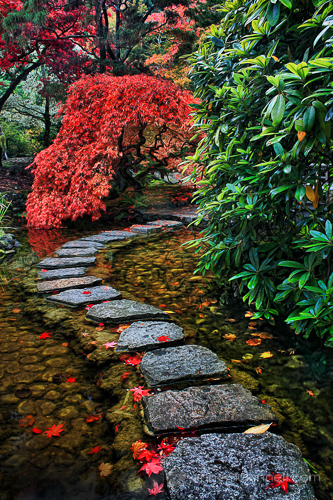
\includegraphics[scale=0.4]{leading_lines1.jpg}
    }
    \subfigure[] {
                \label{fig:leading_lines2}
                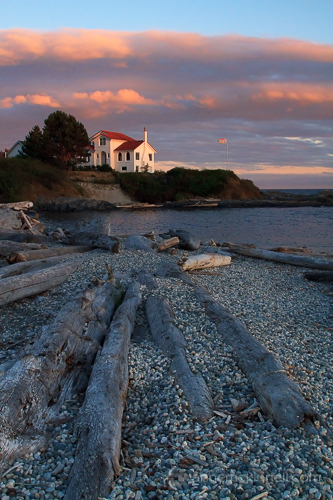
\includegraphics[scale=0.4]{leading_lines2.jpg}
    }
  \caption{Examples of a curved line (a) that redirects the viewer's eye to the maple tree, and vertical lines (b) redirect the subject in the photo.}
  \label{fig:leading_lines_image}
\end{figure}

\subsubsection{Balance of elements}
\label{subsub:balance_elements}

Unconsciously, the human mind evaluates a photo and look if there exists any balance or unbalance between the elements \cite{Santos}.
To judge the balance between the elements of a composition, we must imagine a frame divided by two and a scale that will measure the weight of the left side with the right side.
When the scale is perfectly balanced which is very common in symmetrical images, it means that both sides have the same weight visually, creating what is called static balance.
In dynamic balance, it is possible to create a balance in the image between with two imbalanced sides. This can be achieved if one of the sides has a larger element but the remaining side has a smaller but brighter object.
The scale doesn't have to be perfectly balanced and a strong composition can be created with unbalanced sceneries. This way, the viewers attention will lie over the same side, empowering the subject in the frame.

\todo[inline]{à espera da resposta do autor para fornecer exemplos ilustrativos}


\subsection{Practical Application of Aesthetic Evaluation Systems}
\label{sub:eval_applications}

As referred in Section \ref{sec:photo_eval}, computational aesthetics can be described has aesthetic decisions made by computational methods. Increasing aesthetic awareness, researches developed systems and algorithms that extract and evaluate features of an image based in rules such as the ones described at Section \ref{sub:photo_rules}.

Defining aesthetics as a "concern with beauty and art and understanding of beautiful thing", \citeauthor{Datta} \cite{Datta} described, a system capable of extracting visual properties and automatically tell the difference between aesthetically pleasing and displeasing images. 
Based on a data extracted from an on-line photo sharing community, a set of images and associated aesthetic ratings given by the community, were used to train a classifier.

\todo[inline]{rever parágrafos seguintes}
Obtaining two-dimensional matrices for each of the components and extracted a total of 56 candidate features related to image properties, e.g. exposure, hue, saturation, size and aspect ratio, and composition, e.g. rule of thirds, use of texture and shape convexity. These features were chosen to study patterns that could lead to higher or lower aesthetics ratings. By using a segmentation method based on clustering, information relevant to some features was extracted from objects within the photographs.
From all the candidate features, it was selected a total of 15 visual features that established a significant correlation between the visual properties of photographic images and their aesthetics ratings given by the community. The selected features would later be used by the classifier to attribute a rating to an image.
Later, a publicly accessible system called \emph{ACQUINE} \cite{Datta2010} was developed. A user could upload their photographs and have them rated automatically for aesthetic quality. Compromising on a subset of the features previously presented, \emph{ACQUINE} was able to generate quick responses through a simple interface (Figure \ref{fig:acquine_interface1}) that kept the underlying classifier hidden. A user would then submit an image and wait for the classifiers prediction of aesthetic value. The user could also give a rating on a 7-star scale (Figure \ref{fig:acquine_interface2}) (similar to Photo.net's rating scale) that would be stored for future validation and improvements on the classifier.

\begin{figure}[htbp]
        \centering
    \subfigure[] {
                \label{fig:acquine_interface1}
                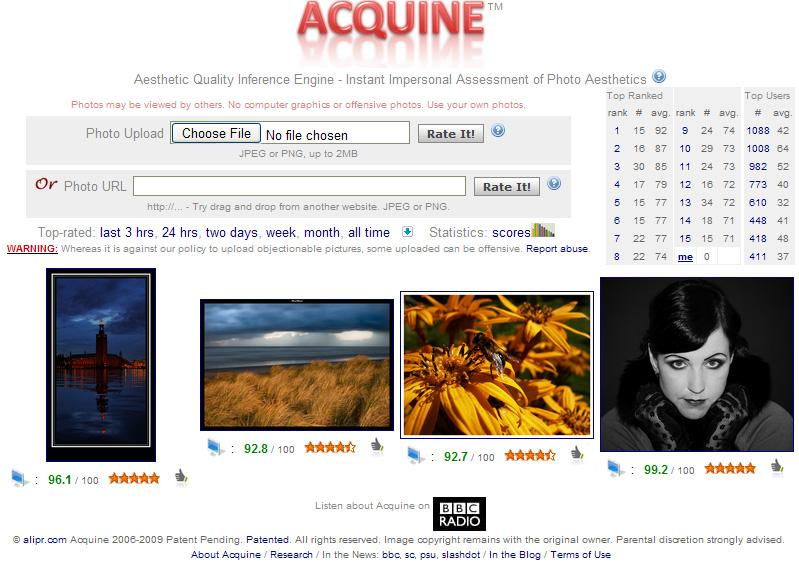
\includegraphics[scale=.4]{acquine_interface1.jpg}
    }
    \subfigure[] {
                \label{fig:acquine_interface2}
                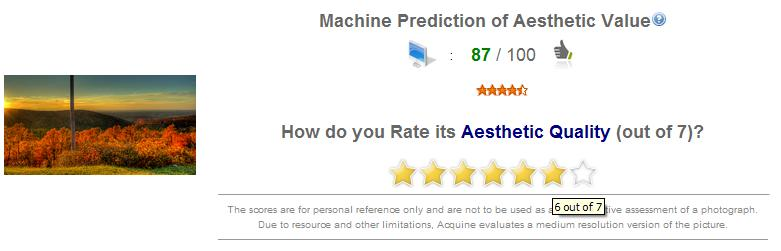
\includegraphics[scale=0.4]{acquine_interface2.jpg}
    }
  \caption{(a) The frontpage of the ACQUINE system, where the users could upload photos. The list of top users on the right side and photos with high ACQUINE aesthetics scores randomly selected at the bottom. (b) Screenshot of the ratings page after a photo upload. \cite{Datta2010}}
  \label{fig:acquine_image}
\end{figure}

Following the same methodology, \citeauthor{Yeh} \cite{Yeh}, described mutable ranking system. This system listed 1000 ranked photographs ordered from the highest rank to the lowest. The score of each photograph was considered as a linear combination of each feature and its corresponding optimal weighting factor, that was found after the extraction of features. However, since the optimal weights might not combine with the users preferences, it enables them to combine personal taste with a trained model, and rearrange the ordered list of ranked photographs.
The weighting adjustments can be feature-based where the user can personally select the weight of each feature (Figure \ref{fig:system_eval1}), or an example-based approach (Figure \ref{fig:system_eval2}), where she selected a photograph they like and have the system update the weighting based on the example chosen.
The features chosen to extract, are quite similar to the ones used in \cite{Datta}, but introduces an interesting composition rule. They extract the subject region and assess the simplicity of a photograph by the colour distribution of the remaining region that corresponds to the background.

\begin{figure}[htbp]
    \centering
    \subfigure[] {
                \label{fig:system_eval1}
                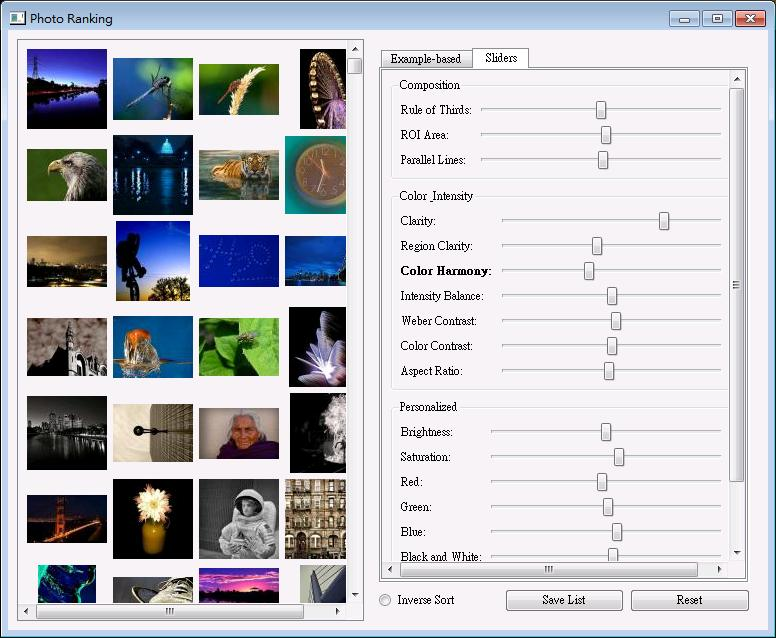
\includegraphics[scale=0.25]{system_eval1.jpg}
    }
    \subfigure[] {
                \label{fig:system_eval2}
                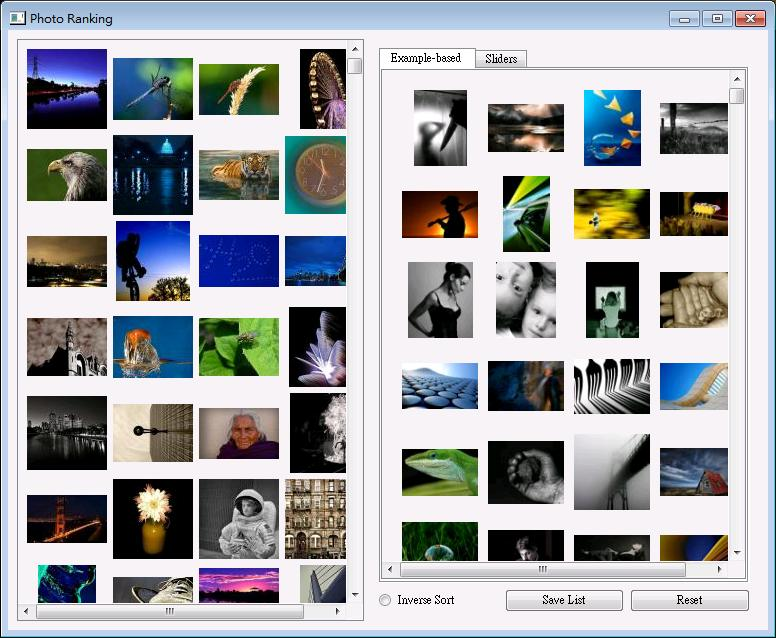
\includegraphics[scale=0.25]{system_eval2.jpg}
    }
  \caption{(a) Re-ranking photographs by adjusting the feature weighting and by (b) selecting a few photographs as example \cite{Yeh}.}
  \label{fig:system_eval_image}
\end{figure}

\section{Computer Vision Algorithms}
\subsection{Keypoint Detection}
\subsubsection{FAST}
\subsubsection{SWIFT}
\subsubsection{SURF}
\subsection{Colour Features}
\subsection{Texture Features}


